\begin{table}[t!]
\begin{center}
\begin{footnotesize}
\begin{tabular}{llll}
\hline
\# & Model & P@1 Val & P@1 Test \\ 
%\hline
%& Baselines & \\
\hline
1	&	Random 			&			25			&  25	\\
2	&	IR Baseline		&			47.2			&	 47	\\
3	&	IR$^{++}$ 		&			50.7$^{**}$			& 36.35	\\
4 & \citet{Iyyer2015}
%\tablefootnote{Our implementation of the architecture described in the paper, using the same embeddings we used with our model and dense layers of equal dimension to our embeddings.} 
& -- & 32.52\\
5 & \citet{khot2017tupleinf} & -- & 46.17 \\
%\hline
%	&	Our Approach & 	&	\\
\hline
6 & Our approach w/o IR	&	50.54$^*$	& 48.66 \\
%7	&	IR$^{++}$ + EF 					&		53.4$^{**\dagger\dagger}$				& 53.4$^{**}$	\\
%8	&	IR$^{++}$ + EF + lexDisc 	&		53.6$^{**\dagger\dagger}$				& 53.42$^{**\dagger}$ 	\\
7	&	Our approach  &	{\bf 54.0}$^{**\dagger\dagger}$		& {\bf 53.3}$^{**\dagger}$ 	\\
\end{tabular}
\end{footnotesize}
%space{-1mm}
\caption{{\footnotesize Performance on the AI2 Kaggle questions, measured by precision-at-one (P@1).  $^*$s  indicate that the difference between the corresponding model and the IR baseline is statistically significant ($^*$ indicates $p < 0.05$ and $^{**}$ indicates $p < 0.001$) and $^{\dagger}$s  indicate significance compared to IR$^{++}$,
%that the difference between the corresponding model and the IR$^{++}$ baseline is statistically significant. %($^\dagger$ corresponds to $p < 0.05$ and $^{\dagger\dagger}$ corresponds to $p < 0.001$).  
All significance values were determined through a one-tailed bootstrap resampling test with 100,000 iterations. }} 
\label{tab:p@1}
\end{center}
\end{table}

\begin{table}[t!]
\begin{center}
\begin{footnotesize}
\begin{tabular}{ll}
\hline
 Ablated Model & P@1 Val \\ 
\hline
 %LO + lexDisc + Emb	&	50.54$^*$ \\
    %Baseline IR$^{++}$ 							&		50.7$^{**}$	\\
	IR$^{++}$ + LO 					&		53.4$^{**\dagger\dagger}$\\
	IR$^{++}$ + LO + lexDisc 	&		53.6$^{**\dagger\dagger}$ \\
    Full Model (IR$^{++}$ + LO + lexDisc + Emb)  &	{\bf 54.0}$^{**\dagger\dagger}$	\\
\end{tabular}
\end{footnotesize}
%space{-1mm}
\caption{{\footnotesize Ablation of feature groups results, measured by precision-at-one (P@1) on validation data.  Significance is indicated as in Table \ref{tab:p@1}.}} 
\label{tab:ablation}
%space{-5mm}
\end{center}
\end{table}

\section{Results}
\label{sec-emnlp2017:results}

Rather than seeking to outperform all other systems at selecting the correct answer to a question, here we aimed to construct a system system that can produce substantially better justifications for why the answer choice is correct to a human user, without unduly sacrificing accuracy on the answer selection task.  Accordingly, we evaluate our system both in terms of it's ability to correctly answer questions (Section \ref{sec-emnlp2017:accuracy}), as well as provide high-quality justifications for those answers (\ref{sec-emnlp2017:justification_results}).  Additionally, we perform an error analysis (Section \ref{sec-emnlp2017:erroranalysis}), taking advantage of the insight the reranked justifications provide into what the model is learning.
% \todo{not sure what this sentence means?}.
% bs: is this clearer?

\subsection{QA Performance}
\label{sec-emnlp2017:accuracy}
We evaluated the accuracy of our system as well as the baselines on the held-out 800 set of test questions.  Performance, measured in precision at 1 (P@1)\cite{manning08}, is shown in Table \ref{tab:p@1} for both the validation (i.e., cross validation on training) and test partitions.  Because NNs are sensitive to initialization, each experimental result shown is the average performance across five runs, each using different random seeds.   

The best performing baseline on the validation data was a model using only IR$^{++}$ features (line 3), but its performance dropped substantially when evaluated on test due to the failure of several random seed initializations to learn.  For this reason, we assessed significance of our model combinations with respect to both the IR baseline as well as the IR$^{++}$ (indicated by $^*$ and $^{\dagger}$s, respectively).
%For this reason, we assessed significance of our model combinations with respect to both the IR baseline (indicated by $^*$) as well as the IR$^{++}$ system (indicated by $^{\dagger}$s).

Our full model that combines IR$^{++}$, lexical overlap, discourse, and embeddings-based features, has a P@1 of 53.3\% (line 7), an absolute gain of 6.3\% over the strong IR baseline despite using the same background knowledge.  
% + LO + lexDisc + Emb\todo{use the text description to make it easier for the reader, e.g. (that combines IR++ with lexical overlap, ...}, has a P@1 of 53.3, an absolute gain of 6.3\% over the strong IR baseline despite using the same background knowledge.  

%\subsubsection{Comparison to Previous Work}
%\begin{flushleft}
%{\bf Comparison to Previous Work}
%space{-1mm}
%\end{flushleft}
\paragraph{Comparison to Previous Work:}
We compared our performance against another model that achieves state of the art performance on a different set of 8th grade science questions, \textsc{TupleInf}(T+T') \citep{khot2017tupleinf}.  \textsc{TupleInf}(T+T') uses Integer Linear Programming to find support for questions via tuple representations of KB sentences\footnote{Notably, one portion of the tuple KB used was constructed based on a different 8th grade question set than the one we use here.}.
%with structured Open IE \citep{Banko2007OpenIE} tuple representations of both questions and knowledge-base sentences to assess how well a given answer choice is entailed or supported.  
On our test data, \textsc{TupleInf}(T+T') achieves 46.17\% P@1 (line 5). 
%\todo{move back to 1 sigdig?}.  
As this model is independent of an IR component, we compare its performance against our full system without the IR-based features (line 6), whose performance is 48.66\% P@1, an absolute improvement of 2.49\% P@1 (5.4\% relative) despite our unstructured text inputs and the far smaller size of our knowledge base (three orders of magnitude). 

%Notably, their KB used by \citeauthor{khot2017tupleinf} is three orders of magnitude larger than ours.  
%Waterloo -- 280GB, ours is SS+QZ -- 72.5MB

\citet{sachan2016science} also tackle the AI2 Kaggle question set with an approach  that learns alignments between questions and structured and semi-structured KB data.
%They reframe the task as answer entailment and learn alignments between structured and semi-structured KB data and the question-answer hypothesis.  
They use only the training questions (splitting them into training, validation, and testing partitions), supplemented by questions found in online study guides, and report an accuracy of 47.84\%.  By way of a loose comparison (since we are evaluating on different data partitions), our model has approximately 5\% higher performance despite our simpler set of features and unstructured KB.  

We also compare our model to our implementation of the basic Deep-Averaged Network (DAN) Architecture of \citet{Iyyer2015}.  %To ensure a more fair comparison, 
We used the same 50-dimensional embeddings in both models, so with the reduced embedding dimension, we reduced the size of each of the DAN dense layer to 50 as well.  For simplicity, we also did not implement their word-dropout, a feature that they reported as providing a performance boost. Using this implementation, the performance on the test set was 31.50\% P@1.  To help with observed overfitting, we tried removing the dense layers and received a small boost to 32.52\% P@1 (line 4).  
The lower performance of their model, which relies exclusively on latent representations of the data, underscores the benefit of including explicit features alongside latent features in a deep-learning approach for this domain.
%This lower performance demonstrates, again, \todo{change to "The lower performance of their model, which relies on latent representations of the data, underscores the relative importance of including both explicit and latent features in a deep-learning solver"?}. the utility of explicit features alongside latent representations in low-data domains.

In comparison to other systems that competed in the Kaggle challenge, our system comes in in 7th place out of 170 competitors (top 4\%).\footnote{Based on the public leaderboard ({\scriptsize \url{https://www.kaggle.com/c/the-allen-ai-science-challenge/leaderboard}}). The best scoring submission had an accuracy of 59.38\%.  Note that for the systems that participated, this set served as \emph{validation} while for us it was test, and thus it is likely that these scores are slightly overfitted to this dataset, but for us it was blind.  As such this is a conservative comparison, and in reality the difference is likely to be smaller.}  Compared with the systems which disclosed their methods, we use a subset of their corpora and substantially less hyperparameter tuning, and yet we achieve competitive results.  
%\todo{count cardal hyperparameters and add}
%bs - removed hyperparam count todo bc it's not straightforward and we're out of space anyway.
%\todo{add paragraph for DAN}

%\subsection{Feature Ablation}
%\begin{flushleft}
%{\bf Feature Ablation }
%space{-2mm}
%\end{flushleft}

\paragraph{Feature Ablation:} To evaluate the contribution of the individual feature groups, we additionally performed an ablation experiment (see Table \ref{tab:ablation}).
Each of our ablated models performed significantly better than the IR baseline on the validation set, including our simplest model, IR$^{++}$+LO.
%\footnote{As we consider the fully ablated IR$^{++}$ to be a baseline, we do not include it here.}.
%, and the version which has the IR-based features removed, LO+lexDisc+Emb.  
   
%The addition of the semi-lexicalized discourse features (lexDisc) did not significantly improve performance over IR$^{++}$+EF, but it did add the stability needed to show significant gains over IR$^{++}$ (compare lines 3 and 5).  
%The addition of the distributional similarity features, which led to our best performing model on the validation data did not improve performance on the test data (line 5), suggesting that while distributional similarity has been shown effective in situations where there is sufficient training data, it struggles to contribute in low-data domains.  Recall that due to over-fitting issues, we fixed our model embeddings, and so while we used domain-specific embeddings, they were not tuned to be task-specific.  We suspect that given more training data we would see much more benefit from these distributional similarity features.


%
% Justification example
%
\begin{table}[t]
\begin{center}
\begin{footnotesize}
%\begin{tabular}{p{1cm}p(6cm}}
\begin{tabularx}{\linewidth}{p{0.7cm}p{6cm}}
\hline
\multicolumn{2}{c}{Question} \\
\hline			
\multicolumn{2}{p{7cm}}{\textbf{Q:} Scientists use ice cores to help predict the impact of future atmospheric changes on climate. Which property of ice cores do these scientists use? } \\
\multicolumn{2}{p{7cm}}{\textbf{A:} The composition of ancient materials trapped in air bubbles} \\
\multicolumn{1}{c}{} & \multicolumn{1}{c}{} \\				
\hline
\multicolumn{1}{l}{Rating} & \multicolumn{1}{c}{Example Justification} \\
\hline			
{\em Good }		&	Ice cores: cylinders of ice that scientist use to study trapped atmospheric gases and particles frozen with in the ice in air bubbles \\
{\em Half }		&	Ice core: sample from the accumulation of snow and ice over many years that have recrystallized and have	trapped air bubbles from previous time periods \\
{\em Topical }	&   Vesicular texture formation [has] trapped air bubbles. \\
{\em Off-topic }	&	Physical change: change during which some properties of material change but ... \\
%\end{tabular}
\end{tabularx}
\end{footnotesize}
\caption{{  Example justifications from the our model and their associated ratings. }} 
\label{tab:justification_examples}
%space{-5mm}
\end{center}
\end{table}

\subsection{Justification Performance}
\label{sec-emnlp2017:justification_results}
One of our key claims is that our approach addresses the related, but more challenging problem of performing \emph{explainable} question answering, i.e., providing a high-quality, compelling justification for the chosen answer.  To evaluate this claim, we evaluated a random set of 100 test questions that both the IR baseline and our full system answered correctly.  For each question, we assessed the quality of each of the top five justifications.  For IR, these were the highest-scoring retrieved documents, and for our system, these were the top-scoring justifications as re-ranked by our model.  Following the methodology of Jansen et al. \citeyear{jansen2017framing}, each justification received a rating of either \emph{Good} (if the connection between the question and correct answer was fully covered), \emph{Half} (if there was a missing link), \emph{Topical} (if the justification was simply of the right topic), or \emph{Off-Topic} (if the justification was completely unrelated to the question). Examples of each rating are provided in Table \ref{tab:justification_examples}.  

\begin{table}[t]
\begin{center}
\begin{footnotesize}
\begin{tabular}{llll}
\hline
 Model 			& Good@1 	& Good@5 	& NDCG@5 \\ 
\hline
IR Baseline 	&	0.52 		&	0.64 		& 0.55 \\
Our Approach & 	{\bf 0.61}	 	&	{\bf 0.74}			& {\bf 0.62}$^{**}$ \\
\end{tabular}
\end{footnotesize}
\caption{{\footnotesize Percentage of questions that have at least one \emph{good} justification within the top 1 (Good@1) and the top 5 (Good@5) justifications, 
%. returned by both the IR baseline and our full model 
as well as the normalized discounted cumulative gain at 5 (NDCG@5) of the ranked justifications.
 Significance indicated as in Table \ref{tab:p@1}.
% returned by each.  
%For NDCG, $^*$  indicates that the difference was significant ($p < 0.001$)
%, as determined through a 1-tailed bootstrap resampling test with 100,000 iterations.
}} 
\label{tab:justification_ndcg}
%space{-5mm}
\end{center}
\end{table}


%\begin{table}[t]
%\begin{center}
%\begin{footnotesize}
%\begin{tabular}{lcc}
%\hline
%% & \multicolumn{5}{c}{\emph{Good}@$k$} \\ 
%Model	& Good@1 & Good@5 \\
%\hline
%IR Baseline 		&	0.52 	&	0.64 \\
%Our Approach 	& 	0.61	 	&	0.74\\
%\end{tabular}
%\end{footnotesize}
%\caption{{\footnotesize Percentage of questions that have at least one \emph{good} justification within the top 1 (Good@1) the top 5 (Good@5) justifications returned by both the IR baseline and our full model.}} 
%\label{tab:justification_performance}
%\end{center}
%\end{table}


%\begin{table}[t]
%\begin{center}
%\begin{footnotesize}
%\begin{tabular}{lccccc}
%\hline
% & \multicolumn{5}{c}{Position Within Top 5} \\ 
%Rating	& 1 & 2 & 3 & 4 & 5\\
%\hline
%\multicolumn{6}{l}{CR Baseline} \\
%\hline
%Good	& 0.52 & 0.42 & 0.39 & 0.35 & \textbf{0.40}\\
%Half		& 0.23 & 0.19 & 0.24 & 0.22 & 0.21\\
%Topical		& 0.18 &0.30 & 0.26 &0.33 & 0.30\\
%Off-Topic	& 0.07 & 0.09 & 0.10 & 0.09 & 0.08\\
%\hline
%\multicolumn{6}{l}{Full Model} \\
%\hline
%Good  &  \textbf{0.61}  &  \textbf{0.54}  &  \textbf{0.43}  &  \textbf{0.40}  &  0.37\\
%Half  &  0.19  &  0.24  &  0.20  &  0.26  &  0.28\\
%Topical  &  0.17  &  0.17  &  0.27  &  0.27  &  0.22\\
%Off-Topic  &  0.02  &  0.05  &  0.09  &  0.06  &  0.12\\
%\end{tabular}
%\end{footnotesize}
%\caption{{\footnotesize Percentage of good, half, topical, and off-topic justifications at each position within the top five justifications returned by both the IR baseline and our full model.}} 
%\label{tab:justification_performance}
%\end{center}
%\end{table}

Results of this analysis are shown using three evaluation metrics in Table \ref{tab:justification_ndcg}.  The first two columns show the percentage of questions which had a \emph{Good} justification at position 1 (Good@1), and within the top 5 (Good@5).  
%justifications with each of the four ratings at each position in the top 5.  
Note that 61\% of the top-ranked justifications from our system were rated as \emph{Good} as compared to 52\% from the IR baseline (a gain of 9\%), despite the systems using identical corpora.  
%In second position, our system had 12\% more \emph{Good} justifications.  

We also evaluated the justification ratings using normalized discounted cumulative gain at 5 (NDCG@5) (as formulated in \citet{manning08}, p.163), where we assigned \emph{Good} justifications a gain of 3.0, \emph{Half} a gain of 2.0, \emph{Topical} a gain of 1.0, and \emph{Off-Topic} a gain of 0.0.  With this formulation, our system had a NDCG@5 of 0.62 while the IR baseline had a significantly lower NDCG@5 of 0.55 ($p < 0.001$), shown in the third column of Table \ref{tab:justification_ndcg}. 

\begin{figure}[t]
\begin{center}
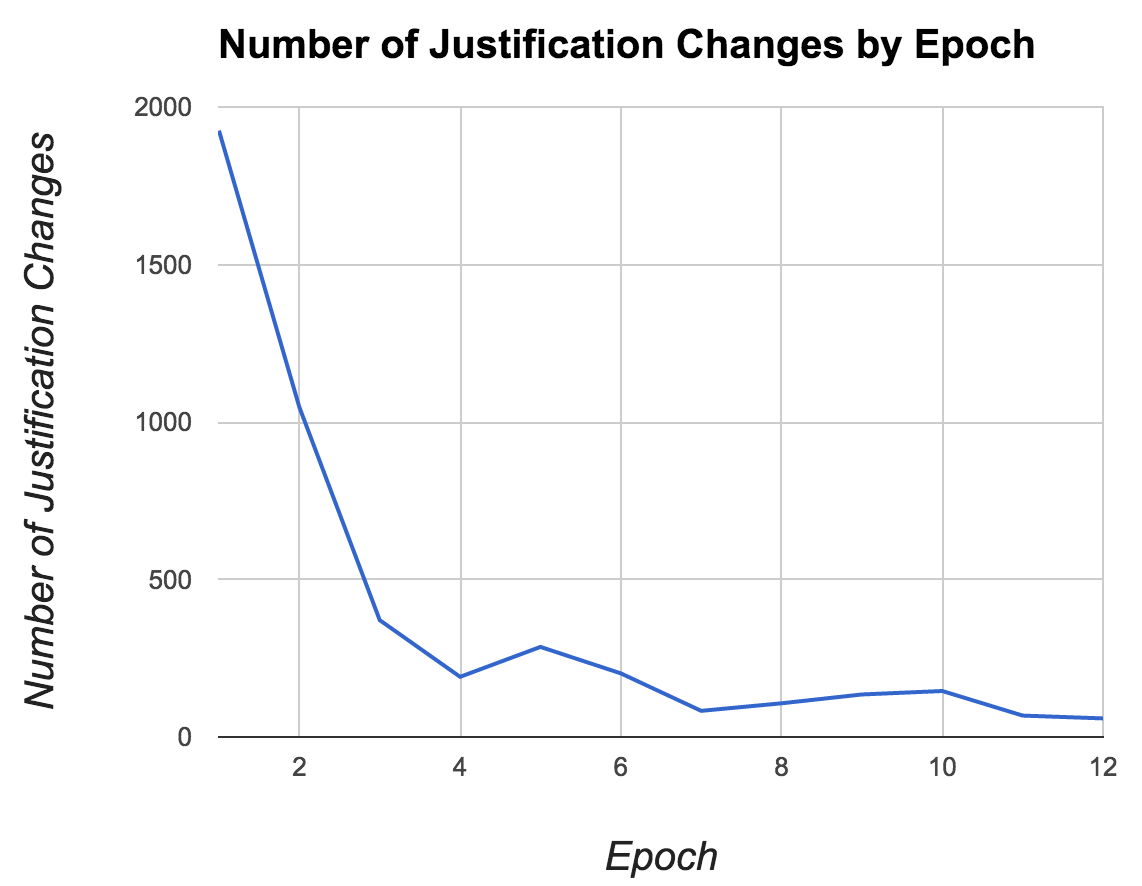
\includegraphics[width=0.8\textwidth]{mainmatter/emnlp2017-qaj/justificationChanges.png}
\caption{Number of questions for which % the IR$^{++}$ + EF + lexDisc + Emb 
our complete model chooses a new justification at each epoch during training.  While this is for a single random seed, we see essentially identical graphs for each random initialization.}
\label{fig:changes}
%space{-5mm}
\end{center}
\end{figure}

%\subsection{Contribution of Jointly Learning to Rank Justifications}
%\begin{flushleft}
%{\bf Contribution of Learning to Rerank Justifications}
%\end{flushleft}
%space{-2mm}
\paragraph{Contribution of Learning to Rerank Justifications:}
The main assertion of this work is that through learning to rank answers and justifications for those answer candidates in an end-to-end manner, we both answer questions correctly and provide compelling justifications as to why the answer is correct.  To confirm that this is the case, we also ran a version of our system that does not re-rank justifications, but uses the top-ranked justification retrieved by IR.  This configuration dropped our performance on test to 48.7\% P@1, a decrease of 4.6\%, and we additionally lose all justification improvements from our system (see Section \ref{sec-emnlp2017:justification_results}), demonstrating that learning this reranking is key to our approach.

Additionally, we tracked the number of times a new justification was chosen by the model as it trained. We found that our system converges to a stable set of justifications during training, shown in Figure \ref{fig:changes}.

%- Demonstrate the need for the latent layer (justifications from IR).


%bs - no room: Greedy is useful: top 1 just vs. top 10 vs. top 100 (OPTIONAL) But we want top 1 anyway.


%\todo{Examples of good/bad questions!?}
%bs: removed todo -- there won't be any room, I promise!

%\todo{Error analysis where it’s doing worse (>= 20+ qs, where our got it wrong) -- 20 questions we got wrong, find top 2 places we went wrong (half a column}

%
%\begin{table}[!th]
%\begin{center}
%\begin{footnotesize}
%\hfill
%\begin{tabular}{ll}
%\hline
%Error Type & Percent \\ 
%\hline
%Short justification/High lexical overlap  & 53.3\%\\
%Complex inference required   & 43.3\% \\
%Knowledge Base Noise  & 6.7\% \\
%Word order necessary	 & 6.7\% \\
%Coverage & 6.7\% \\
%Negation	& 3.3\% \\
%Other & 6.7\% \\
%\end{tabular}
%\end{footnotesize}
%\caption{{\footnotesize Summary of the findings of the 30 question error analysis.  
%%Examples of several categories provided in separate tables. 
%Note that a given question may fall into more than one category.}} 
%\label{tab:erroranalysis}
%\vspace{-5mm}
%\end{center}
%\end{table}
%
%%\begin{table}[!th]
%%\begin{center}
%%\begin{footnotesize}
%%\hfill
%%\begin{tabular}{p{0.8cm}p{6.5cm}p{1cm}}
%%\hline
%%\multicolumn{2}{l}{Error Type} & Percent \\ 
%%\hline
%%\multicolumn{2}{l}{\textbf{Shorter justification with lots of lexical overlap}} & 53.3\%\\
%%\multicolumn{2}{l}{\textbf{Complex inference required}}  & 43.3\% \\
%%\hline
%%
%%\\
%%\hline
%%\multicolumn{2}{l}{\textbf{KB Noise}}  & 6.7\% \\
%%\hline
%%Question: & \multicolumn{2}{p{7.5cm}}{ If an object traveling to the right is acted upon by an unbalanced force from behind it  the object will}	\\
%%Correct: & \multicolumn{2}{p{7.5cm}}{speed up }	\\
%%Chosen & \multicolumn{2}{p{7.5cm}}{ change direction }	\\
%%			& \multicolumn{2}{p{7.5cm}}{\textit{ Unbalanced force: force that acts on an object that will change its direction}}	\\
%%%\hline
%%\multicolumn{3}{p{8cm}}{The system found a sentence in the knowledge base that "justifies" the correct answer.}	\\
%%%
%%\\
%%\hline
%%\multicolumn{2}{l}{\textbf{Word order necessary}}	 & 6.7\% \\
%%\hline
%%Question: & \multicolumn{2}{p{7.5cm}}{ The acceleration of a small rocket that has just been launched can be quantitatively found by}	\\
%%Correct: & \multicolumn{2}{p{7.5cm}}{dividing the force acting upon the rocket by its mass }	\\
%%Chosen & \multicolumn{2}{p{7.5cm}}{ dividing the mass of the rocket by the force acting upon it }	\\
%%			& \multicolumn{2}{p{7.5cm}}{\textit{ (same for both) acceleration: force divided by mass}}	\\
%%%\hline
%%\multicolumn{3}{p{8cm}}{The ordering of the answer choice terms was necessary for answering the question.}	\\
%%%
%%\\
%%\hline
%%\multicolumn{2}{l}{\textbf{Coverage}} & 6.7\% \\
%%\hline
%%Question: & \multicolumn{2}{p{7.5cm}}{ Which activity most effectively ensures the proper functioning of osteocytes?}	\\
%%Correct: & \multicolumn{2}{p{7.5cm}}{consuming mineral-rich foods}\\
%%			& \multicolumn{2}{p{7.5cm}}{\textit{ most lipids consumed from food are in the form of triglycerids}}	\\	
%%Chosen & \multicolumn{2}{p{7.5cm}}{increasing the respiratory rate }	\\
%%			& \multicolumn{2}{p{7.5cm}}{\textit{ hyperventilation increased respiratory rate}}	\\
%%%\hline
%%\multicolumn{3}{p{8cm}}{The knowledge base had no coverage for the concept of \emph{osteocyte}, so the system grasped at proverbial straws.}	\\
%%%
%%\\
%%\hline
%%\multicolumn{2}{l}{\textbf{Negation}}	& 3.3\% \\
%%\hline
%%%\multicolumn{3}{l}{Example}	\\
%%Question: & \multicolumn{2}{p{7.5cm}}{ Which feature does not form as a result of tectonic plates diverging?}	\\
%%Chosen: & \multicolumn{2}{p{7.5cm}}{ rift valley }	\\
%%			& \multicolumn{2}{p{7.5cm}}{\textit{ Rift valley: deep valley formed as tectonic plates move apart. }}	\\
%%\multicolumn{3}{p{8cm}}{Note that the justification actually shows that the chosen answer is incorrect, rather than justifying it.  This is the expected behavior for the system for these negated questions as we don't handle them differently.}	\\
%%%
%%\\
%%\hline
%%\multicolumn{2}{l}{\textbf{Other}} & 6.7\% \\
%%\end{tabular}
%%\hfill
%%\end{footnotesize}
%%\caption{{\footnotesize Summary of the findings of the 30 question error analysis.  Note that a given question may fall into more than one category.}} 
%%\label{tab:erroranalysis}
%%\end{center}
%%\end{table}
%
%\begin{table}[t]
%\begin{center}
%\begin{footnotesize}
%\begin{tabular}{p{1cm}p{6cm}}
%\hline
%Type: & \textbf{Short justification/High lexical overlap}\\
%\hline
%Question: & The length of time between night and day on Earth varies throughout the year. This time variance is explained primarily by $\rule{1cm}{0.15mm}$. \\
%Correct: & Earth 's angle of tilt \\
%			 & \textit{ ... the days are very short in the winter because the sun's rays hit the earth at an extreme angle ... due to the tilt of the earth's axis. } \\
%Chosen: &  Earth 's distance from the Sun \\
%			& \textit{ Is light year time or distance? Distance}	\\
%\end{tabular}
%\hfill
%\end{footnotesize}
%\caption{{\footnotesize Example of the system preferring a justification for which all the terms were found in either the question or answer candidate.
%% while the justification for the correct answer contained additional information necessary to fully explain the answer. 
%(Justifications shown in italics)
%}} 
%\label{tab:ex_lex_overlap}
%\vspace{-5mm}
%\end{center}
%\end{table}
%
%\subsection{Error Analysis}
%\label{sec-emnlp2017:erroranalysis}
%
%%\todo{provide examples for all without other -- make full width}
%
%
%To better understand the limitations of our current system, we performed an error analysis of 30 incorrectly answered questions.  %Taking advantage of the ability of the chosen justifications to provide insight into what the system found important, we 
%We examined the top 5 justifications returned for both the correct and chosen answers.  
%%Among the questions analyzed we found some interesting trends.   
%Notably, 50\% of the questions analyzed had one or more good justifications in the top 5 returned by our system, but for a variety of reasons, summarized in Table \ref{tab:erroranalysis}, the system incorrectly ranked another answer's justification higher.  
%
%The most common form of error was the systems preference 
%was when the chosen answer's justification contained a 
%for short justifications with a large degree of lexical overlap with the question and answer choice itself, 
%%with few unmatched terms, 
% shown by the example in Table \ref{tab:ex_lex_overlap}.  
% %This effect was magnified when the correct answer required more "explanation" to connect the question to the answer.  
%This suggests that the system has learned that generally many unmatched words are indicative of an incorrect answer.  While this may typically be true, extending the system to be able to prefer the \emph{opposite} with certain types of questions would potentially help with these errors.  
%
%The second largest source of errors came from questions requiring complex inference (causal, process, quantitative, or model-based  reasoning) as with the question:%.  For example, to answer the question:
% %\begin{quote}
%\begin{addmargin}[1em]{2em}% 1em left, 2em right 
% \begin{footnotesize}
%  \textit{Q: Mr. Harris mows his lawn ...[and leaves] the clippings on the ground. Which long term effect will this most likely have on his lawn? \\
%  A: It will provide the lawn with needed nutrients.}
% \end{footnotesize}
%%\end{quote}
%\end{addmargin}
%To answer this, you would need to link together: \textit{cut grass left on the ground $\rightarrow$ grass decomposes $\rightarrow$ decomposed material provides nutrients}. 
%These questions constitute a large portion of our errors,  
%%is a large set of questions that our system is not particularly designed to handle, 
%demonstrating not only the difficulty of the question set but also the need for systems that can robustly handle a variety of question types and their corresponding information needs.  
%
%Aside from these main groups, there were some smaller trends:  
%7\% of the incorrectly chosen answers actually had justifications which "validated" them due to noise in the knowledge base, 7\% required word-order to answer (e.g., \emph{mass divided by acceleration} vs. \emph{acceleration divided by mass}), another 7\% of questions suffered from lack of coverage of the question concept in the knowledge base,
%%(see example in Table \ref{tab:ex_coverage}), 
% and 3\% failed to appropriately handle negation (i.e., questions of the format \emph{Which of the following are NOT ...}). 
%
%
%
%% bs: no room: - Negative results?


%\begin{table}[t]
%\begin{center}
%\begin{footnotesize}
%\begin{tabular}{p{1cm}p{6cm}}
%\hline
%Type: & \textbf{Coverage}\\
%\hline
%Question: & Which activity most effectively ensures the proper functioning of osteocytes? \\
%Correct: & consuming mineral-rich foods\\
%			& \textit{ most lipids consumed from food are in the form of triglycerids}	\\	
%Chosen & increasing the respiratory rate 	\\
%			& \textit{ hyperventilation increased respiratory rate}	\\
%\end{tabular}
%\hfill
%\end{footnotesize}
%\caption{{\footnotesize Example of a question for which coverage was an issue.  The KB had no coverage for the concept of \emph{osteocyte}.}} % , so the system grasped at proverbial straws.}} 
%\label{tab:ex_coverage}
%\end{center}
%\end{table}


%\begin{table}[!th]
%\begin{center}
%\begin{footnotesize}
%\begin{tabular}{p{1cm}p{6cm}}
%\hline
%Type: & \textbf{Complex inference required}\\
%\hline
%Question: & Mr. Harris mows his lawn twice each month. He claims that it is better to leave the clippings on the ground. Which long term effect will this most likely have on his lawn? \\
%Correct: &  It will provide the lawn with needed nutrients. 	\\
%\end{tabular}
%\hfill
%\end{footnotesize}
%\caption{{\footnotesize Example of a question for which complex inference is required.  In order to answer the question, you would need to assemble the following chain of events: cut grass left on the ground $\rightarrow$ grass decomposes $\rightarrow$ decomposed material provides nutrients.}} 
%\label{tab:ex_complex_inf}
%\end{center}
%\end{table}

